\documentclass[14pt]{beamer}
\title{FUTOSHIKI PUZZLE SOLVER}
\author[BVRIRH]{Mounika D: 19WH1A05A0: CSE-B \\ Srija K: 19WH1A0585: CSE-B \\ Akshitha R: 19WH1A0404: ECE-A \\Srija A: 19WH1A0233: EEE \\Aparna P: 19WH1A1228: IT-A}
\date{5 April, 2021}
\usepackage{hyperref}
\usepackage{graphicx}
\beamertemplateballitem

\begin{document}
    \begin{frame}
        \titlepage
          \begin{center}
             \small{BVRIT Hyderabad College of Engineering for Women}
          \end{center}
    \end{frame}
    \begin{frame}
        \frametitle{Introduction}
        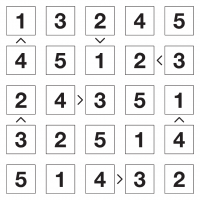
\includegraphics[width=6cm]{puzzle_photo.png}
    \end{frame}
    \begin{frame}
        \frametitle{Approach}
        \begin{itemize}
            \item Taking puzzle as input
            \item Processing it and giving solution to the user
        \end{itemize}
    \end{frame}
    \begin{frame}
        \frametitle{Challenges}
        \begin{itemize}
            \item Disobeying inequalities
            \item Making our code generalized
            \item Pushing files into git
        \end{itemize}
    \end{frame}
    \begin{frame}
          \frametitle{Learnings}
          \begin{itemize}
              \item{Latex}
              \item{Gitlab}
              \item{Team Work}
              \item{Self learning}
          \end{itemize}
    \end{frame}
    \begin{frame}
        \frametitle{Tech Stack}
        \begin{itemize}
           \item OS : Windows 10, Ubuntu 16.04
           \item Language : Python 3.7.2
           \item Latex, Gitlab
        \end{itemize}
    \end{frame}
    \begin{frame}
         \frametitle{GIT}
              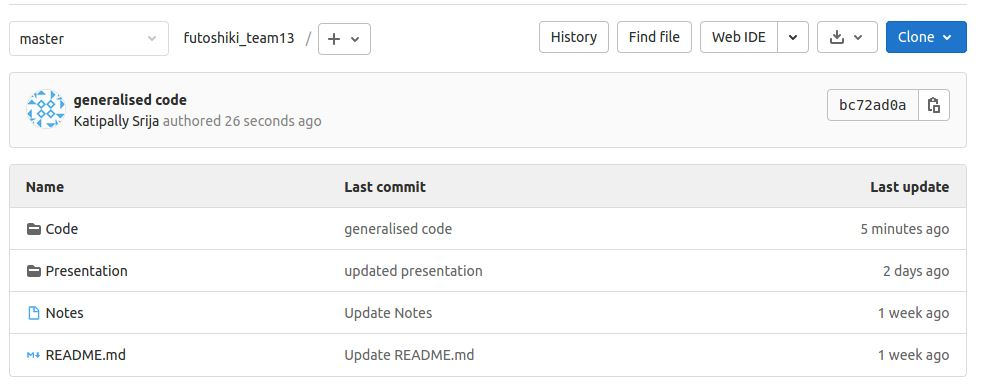
\includegraphics[width=10cm]{git_img.jpeg}
    \end{frame}
    \begin{frame}
         \frametitle{Demo}
             \vspace{0.1in}
             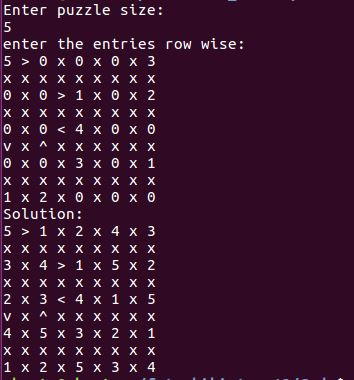
\includegraphics[width=5cm]{output1.jpeg}
             \vspace{1.3in}
             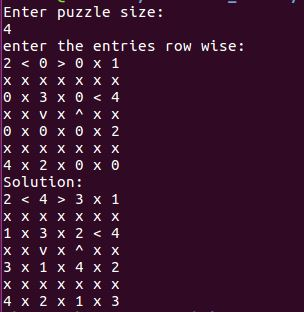
\includegraphics[width=5cm]{output2.jpeg}
    \end{frame}
    \begin{frame}
         \frametitle{Statistics}
            \begin{itemize}
               \item Total lines of code : 109
               \item Total functions : 15
               \item Commits: 61
            \end{itemize}
    \end{frame}
    \begin{frame}
        \begin{center}
             Thank you!!!
        \end{center}
    \end{frame}
\end{document}
            

                                                                                                                                                                                          1,1           Top

